\chapter{Preliminaries}

In this chapter we present the mathematical background used in this thesis. Step by step we progress towards the construction and meaning of the GIT fan. The first section covers the notion of algebraic group actions which lead to various concepts of quotients introduced in the second section. Afterwards, we provide the details for constructing GIT quotients according to Mumford \cite{git}. Finally, a concrete description of available GIT quotients w.r.t. to torus actions in terms of a quasifan is given. Computing this quasifan constitutes the main part of the thesis.

For the remainder of this chapter let $\field$ be an algebraically closed field.

%Gröbnerbasen, Buchberger

\section{Algebraic group actions}

In this section we extend the notion of groups acting on sets to actions on objects in algebraic geometry. We only cover the case of affine varieties here. For a more general approach considering pre\=/schemes, see \cite{git}. Broadly speaking, we require the the group and the set operated on to carry structures of affine varieties such that the set\=/theoretical group action becomes a morphism.

\begin{defi}[Actions of affine algebraic groups]
	An \emph{affine algebraic group} $G$ is an affine variety together with a morphism $m\colon G \times G \rightarrow G$ such that $G$ carries a group structure with the group law $m$. A \emph{homomorphism} of algebraic groups $G$ and $H$ is a morphism $f\colon G \rightarrow H$ such that $f$ preserves the group structure.
\end{defi}

\begin{ex}
	\label{example:algebraic_torus}
	The affine variety $$(\field^*)^n \cong V(t_1t_1^{-1} - 1,\dots, t_nt_n^{-1}-1)\subseteq\field[t_1,t_1^{-1},...,t_n,t_n^{-1}]$$
	is an affine algebraic group via the group law
	$$m\colon (\field^*)^n \times (\field^*)^n \rightarrow (\field^*)^n,\quad ((r_1,\dots,r_n),(s_1,\dots,s_n)) \mapsto (r_1s_1,\dots,r_ns_n).$$
	Note that $m$ is polynomial when formulated over $\field[t_1,t_1^{-1},...,t_n,t_n^{-1}]$.
	
	We claim that its comultiplication $m^*$, that is the pullback of the multiplication $m$, is given by
	$$\O((\field^*)^n) \rightarrow \O((\field^*)^n) \tensor \O((\field^*)^n),\quad \mathbf{t}^\alpha \mapsto \mathbf{t}^\alpha \tensor \mathbf{t}^\alpha,\quad \forall \alpha\in\integer^n.$$
	Clearly, this is a $\field$\=/algebra homormophism. It suffices to check equality with $m^*$ on a set of generators $\{\mathbf{t}^\alpha\mid \alpha\in\integer^n\}$. Now, 
	$$\mathbf{t}^\alpha \tensor \mathbf{t}^\alpha (P, Q) = P^\alpha\cdot Q^\alpha = (PQ)^\alpha =  (\mathbf{t}^\alpha \circ m) (P,Q) = m^*(\mathbf{t}^\alpha) (P,Q)$$ holds for all $\alpha\in\integer^n$ and $P,Q\in(\field^*)^n$. The claim follows.
\end{ex}

\begin{defi}
	An affine algebraic group $G$ is called \emph{(algebraic) torus of dimension $n$} iff there exists $n>0$ such that $G$ is isomorphic to the affine algebraic group $(\field^*)^n$.
\end{defi}

%\begin{remark}
%	\label{remark:torus_from_integral_vectors}
%	Let $\field$ be a algebraically closed field of characteristic zero. Then any finite set $\{v_1,\dots,v_r\}\subseteq\integer^k$ of integral vectors constitutes an algebraic torus of the same dimension as the linear subspace $L = \langle v_1,\dots,v_r\rangle_\rational$. Denote the dimension of $L$ by $d$. Then there exists an $\rational$-linear isomorphism such that $L\cong \rational^d$. In particular, this isomorphism translates to a $\field$\=/algebra isomorphism $\field[L] \cong \field[\rational^d]$ when $\rational$ is embedded into $\field$ as its prime field.
%	It follows that $\spec(\field[L])$ is an algebraic torus via
%	$$\spec(\field[L]) \cong \spec(\field[\rational^d]) =(\field^*)^d.$$
%\end{remark}

\begin{defi}[Algebraic Group action]
	Let $G$ be an affine algebraic group and $X$ be an affine variety. An (algebraic) group action of $G$ on $X$, denoted by $G\acts X$, is a morphism $\varphi\colon G\times X \rightarrow X$ such that $\varphi$ defines a set\=/theoretic group action of $G$ on $X$ via
	$$g\cdot x \defeq \varphi(g,x).$$
\end{defi}

%\begin{ex}
%	\label{example:torus_group_action}
%	Let $X = V(\ideal)\subseteq\field[x_1,\dots,x_r]$ be an affine variety such that its coordinate ring permits a $\integer^k$\=/grading. This grading extends to a $\integer^k$\=/grading of $\field[\mathbf{x}]$  via
%	$$\deg(x_i) \defeq \deg(\overline{x_i})\quad 1\leq i \leq r$$
%	so that $\ideal$ becomes homogeneous. The map
%	$$*\colon(\field^*)^k \times X \rightarrow X,\quad (t,P) \mapsto (t^{q_1}P_1,\dots,t^{q_r}P_r)$$
%	defines a group action. Clearly, the function is polynomial and the identity and compatibility axioms hold. It remains to check that it is well defined. Since we have $f(t*P) = t^q f(P)$ for all homogeneous polynomials $f$ of degree $q\in\integer^k$, for any point $P$ vanishing on the homogeneous ideal $\ideal$, $t*P$ also vanishes on $\ideal$.
%\end{ex}

\begin{construction}
	\label{construction:algebraic_torus}
	We give a concrete description of an algebraic torus $T$ of dimension $n$ acting on an affine variety $X$ via a morphism $\varphi\colon G\times X \rightarrow X$. It will turn out that group actions of $n$\=/dimensional tori on $X$ correspond to $\integer^n$ gradings on $\O(X)$.
	
	W.l.o.g. assume that $T = (\field^*)^n$ with the group law $m$ as specified in Example~\ref{example:algebraic_torus}. Note that the regular functions of $T$ are given by $\field[\mathbf{t},\mathbf{t}^{-1}]$ and the comultiplication $\varphi^*$ is injective since any regular function of $X$ vanishing on $GX$ also vanishes on $X$ by the identity axiom. Furthermore, we have $$\O(T)\tensor\O(T)\tensor\O(X)\cong\O(X)[\mathbf{t},\mathbf{t}^{-1},\mathbf{u},\mathbf{u}^{-1}]\quad\text{via}\quad\mathbf{t}^\alpha \tensor \mathbf{t}^\beta \tensor f \mapsto f\mathbf{t}^\alpha\mathbf{u}^\beta.$$
	For $\alpha\in\integer^n$, define
	$$\O(X)_\alpha \defeq \{f\in\O(X)\mid \varphi^*(f) = \mathbf{t}^\alpha \tensor f\},$$
	which is a submodule of $\O(X)$. Let $\sum_{\alpha\in I} f_\alpha$ be a finite linear combination of zero with $f_\alpha\in\O(X)_\alpha$. It follows that
	$$0 = \varphi^*(0) = \varphi^*\left(\sum_{\alpha\in I} f_\alpha\right) = \sum_{\alpha\in I} \varphi^*(f_\alpha) = \sum_{\alpha\in I} \mathbf{t}^\alpha \tensor f_\alpha.$$
	Coefficient comparison in $\O(X)[\mathbf{t},\mathbf{t}^{-1},\mathbf{u},\mathbf{u}^{-1}]$ shows that $f_\alpha = 0$. Hence, the sum
	$$\bigoplus_{\alpha\in\integer^n} \O(X)_\alpha \subseteqq \O(X)$$
	is direct.

	Let $f\in \O(X)$ and write $\varphi^*(f)$ as a finite linear combination
	$$\varphi^*(f) = \sum_{\alpha\in I} \mathbf{t}^\alpha \tensor f_\alpha.$$
	When moving to $\field$\=/algebra homomorphisms, the compatibility axiom translates to
	$$(m^* \tensor \id_{\O(X)}) \circ \varphi^* = (\id_{\O(T)} \tensor \varphi^*) \circ \varphi^*.$$
	Hence, we obtain
	$$\sum_{\alpha\in I} \mathbf{t}^\alpha \tensor \mathbf{t}^\alpha \tensor f_\alpha = (m^* \tensor \id_{\O(X)}) \circ \varphi^*(f) =  (\id_{\O(T)} \tensor \varphi^*) \circ \varphi^*(f) = \sum_{\alpha\in I}\mathbf{t}^\alpha \tensor \varphi^*(f_\alpha).$$
	Comparing coefficients yields $\varphi^*(f_\alpha) = \mathbf{t}^\alpha \otimes f_\alpha$, that is $f_\alpha\in \O(X)_\alpha$. Furthermore,
	$$\varphi^*\left(\sum_{\alpha\in I} f_\alpha\right) = \sum_{\alpha\in I} \varphi^*(f_\alpha) = \sum_{\alpha\in I} \mathbf{t}^\alpha \tensor f_\alpha = \varphi^*(f).$$
	$\varphi^*$ being injective implies that
	$$f = \sum_{\alpha\in I} f_\alpha,$$
	proving that
	$$\bigoplus_{\alpha\in\integer^n} \O(X)_\alpha = \O(X).$$
	Since $\varphi^*$ preserves the multiplication of $\O(X)$, it holds that $\O(X)_\alpha \O(X)_\beta \subseteq \O(X)_{\alpha+\beta}$. Hence, $\O(X)$ becomes a $\integer^n$\=/graded $\field$\=/algebra. Conversely, every $\integer^n$\=/grading on $\O(X)$ determines a group action $\psi$ of $T$ on $X$ with the corresponding coaction defined by 
	$$\psi^*(f) = \mathbf{t}^{\deg(f)}\tensor f\quad \forall f\in\O(X)\ \mathrm{homogeneous}.$$
	
	By taking a finite set $\{g_1,\dots,g_m\}$ of $\integer^n$\=/homogeneous generators of $\O(X)$, we obtain an embedding $X\subseteq\field^m$ such that the vanishing ideal $\ideal \defeq I(X)\subseteq\field[x_1,\dots,x_m]$ of $X$ is homogeneous w.r.t. the grading
	$$\deg(x_i) = \deg(g_i)\in\integer^n$$
	on $\field[x_1,\dots,x_m]$.
	By construction, we have $\varphi^*(g_i) = \mathbf{t}^{\deg(g_i)} \tensor g_i$ which translates to the coaction  $\psi^*(x_i) = \mathbf{t}^{\deg(g_i)} \tensor x_i$ in $\field[x_1,\dots,x_m] / \ideal$.
	The group action is recovered as follows:
	$$T \times X \longrightarrow X,\quad (t,P) \mapsto (\psi^*(x_1)(t,P),\dots,\psi^*(x_m)(t,P)) = (t^{\deg(g_1)}P_1,\dots,t^{\deg(g_m)}P_m).$$
	
	We conclude that any action of a torus of dimension $n$ on an affine variety $X$ may be described by a set of integral vectors $q_i\in\integer^n$, $1\leq i \leq m$, and a suitable embedding of $X$ in $\field^m$ such that its vanishing ideal is homogeneous w.r.t.
	$$\deg(x_i) = q_i,\quad 1\leq i \leq m.$$
	The group action is given by
	$$(\field^*)^n \times X \longrightarrow X,\quad (t,P) \mapsto (t^{q_1}P_1,\dots,t^{q_m}P_m).$$
\end{construction}

\begin{remark}
	Let $G$ be an affine algebraic group acting on an affine variety $X$. Let $x\in X$. The stabiliser subgroup $G_x$ is a closed, affine subvariety since it is the preimage of the closed point $\{x\}$ of the morphism $g\mapsto gx$. It follows that $G_x$ is an affine algebraic subgroup.
\end{remark}

\begin{remark}[Group action on regular functions]
	If $\varphi$ is a group action of an affine algebraic group $G$ on an affine variety $X$, we obtain a group action of $G$ on the regular functions $K(X)$ of $X$ by
	$$G\times K(X)\rightarrow K(X), \quad(g,\frac{f}{h}) \mapsto \frac{f\circ \varphi(g^{-1},\wildcard)}{h\circ \varphi(g^{-1},\wildcard)}\ .$$
	
	If $U$ is a $G$\=/invariant open subset of $X$, that is $GU = G$, the restriction of $G\acts K(X)$ to $\O_X(U)$ yields a group action $G\acts\O_X(U)$. Note that if the denominator $h$ does not vanish on any point in $U$, then the same holds for $h\circ \varphi(g^{-1},\wildcard)$ as we have $$\varphi(g^{-1},\wildcard)(U) \subseteq GU = U.$$
	
	We say that $f\in\O_X(U)$ is \emph{$G$\=/invariant} iff $gf = f$ holds for all $g\in G$. The subalgebra of $G$\=/invariant functions is denoted by $\O_X(U)^G$.
	\index{OXUG@$\O_X(U)^G$}%
\end{remark}

\begin{ex}
	\label{example:regular_functions_torus_group_action}
	Consider an algebraic group action $\varphi\colon T \rightarrow X$ of a torus $T$ of dimension $n$ on an affine variety $X$. By Construction~\ref{construction:algebraic_torus}, $\O(X)$ is a $\integer^n$\=/graded $\field$\=/algebra. For any homogeneous $f\in\O(X)$ and $g\in (\field^*)^n$, we have
	$$(g^{-1}f)(x) = f \circ \varphi(g,x) = \varphi^*(f)(g,x) = (\mathbf{t}^{\deg(f)} \tensor f)(g,x) = g^{\deg(f)}\cdot f(x)\quad \forall x\in X.$$
	In particular, it is easy to see that
	$$g^{-1}f = g^\alpha f\quad \forall g\in (\field^*)^n \ \Longleftrightarrow \ f\in\O(X)_\alpha,$$
	where $\alpha\in\integer^n$, the left multiplication is given by the group action and the right one is the scalar multiplication of $\O(X)$ as $\field$\=/module.
	For this reason it follows that
	$$ \O(X)^T = \O(X)_0.$$
\end{ex}

\section{Good quotients}
When an algebraic group $G$ acts on an affine variety $X$, naturally one questions if the orbit space $X/G$ defined by the group action can be equipped with the structure of an variety such that the quotient map $p\colon X\rightarrow X/G$ becomes a morphism. Consider the following example.

\begin{ex}
	\label{example:bad_quotient}
	Let $G=\complex^*$ be a one dimensional algebraic torus action on the affine variety $X = \complex^2$ via scaling, that is
	$$(t,(x_1,x_2)) \mapsto (tx_1,tx_2).$$
	Each line $l$ through the origin in $\complex^2$ yields an orbit when removing 0. The origin point is $G$\=/invariant and thus an orbit on its own.
	If the set\=/theoretical quotient map $p$ would be a morphism, a regular function $\varphi$ in $\O(X/G)$ induces a regular function $\psi = \varphi \circ p$ in $\O(X)$ that is $G$\=/invariant. In particular, $\psi$ has to be constant on the closure of each orbit. Since each closure contains the origin, $\psi$ and thus $\varphi$ have to be constant. It follows that $\O(X/G) \cong \field$, contradicting $|X/G| > 1$. Consequently, the set\=/theoretical quotient map is no good quotient in the following sense.
\end{ex}

\begin{defi}[Good quotient, \phantom{}{\cite[Definition 5.0.5]{cls}}]
	Let $G$ be an affine algebraic group acting on an affine variety $X$. A $G$\=/invariant morphism $p\colon X \rightarrow Y$ is called a \emph{good (categorial) quotient}, if
	\begin{enumerate}[label={\upshape(\roman*)}]
		\item the pullback $p^*\colon \O_Y \rightarrow (p^*\O_X)^G$ is an isomorphism of sheaves, that is, for any open $U\subseteq X$ the pullback $p^*\colon \O_Y(U) \rightarrow \O_X(p^{-1}(U))^G$ is an isomorphism of $\field$\=/algebras (note that preimages of $p$ are $G$\=/invariant),
		\item $p(W)$ is closed for any $G$\=/invariant, closed $W\subseteq X$,
		\item the images of disjoint $G$\=/invariant, closed subsets are disjoint.
	\end{enumerate}
\end{defi}

If $\O(X)^G$ is finitely generated, the canonical embedding $\O(X)^G \hookrightarrow \O(X)$ yields a good quotient $p\colon X \rightarrow Y$, where $Y$ is the affine variety with coordinate ring $\O(X)^G$. The question of $\O(X)^G$ being finitely generated is addressed by Hilbert's fourteenth problem and has been answered negatively by Nagata. \cite[chapter 4]{lectures_invariant_theory}

Good quotients admit the following useful properties.

\begin{prop}[\phantom{}{\cite[Theorem 5.0.6 \& Proposition 5.0.7]{cls}}]
	\label{prop:good_quotient_properties}
	Let $G, X$ be as above. Let $p\colon X \rightarrow Y$ be a good quotient. Then it holds that
	\begin{enumerate}[label={\upshape(\roman*)}]
		\item $p$ is surjective,
		\item for any $G$\=/invariant morphism $\varphi\colon X \rightarrow Z$, there exists a unique morphism $\psi\colon Y \rightarrow Z$ such that $\varphi = \psi \circ p$,
		\label{enum_item:good_quotient_universal_property}
		\item the topology on $Y$ coincides with the quotient topology induced by $p$,
		\item $p$ separates closed $G$\=/orbits, that is
		$$p(x) \neq p(y)\ \Leftrightarrow\ \overline{Gx}\cap\overline{Gy} = \emptyset$$
		for all points $x,y\in X$.
		\item Each fibre of $p$ contains a unique closed G\=/orbit. In particular, $p$ induces a bijection
		$$\{Gx\mid x\in X\ \mathrm{such}\ \mathrm{that}\ Gx = \overline{Gx}\}\simeq Y.$$
		\label{enum_item:good_quotient_space_bijection_closed_orbits}
	\end{enumerate}
\end{prop}

Indeed, good quotients are categorical quotients by \ref{enum_item:good_quotient_universal_property} and the good quotient space $Y$ is unique up to isomorphism. For this reason we also write $X\sslash G$ for $Y$.
\index{X//G@$X\sslash G$}%
Note that by \ref{enum_item:good_quotient_space_bijection_closed_orbits}, in general $X\sslash G$ does not coincide with the orbit space $X / G$ as we loose all non\=/closed orbits. In the setting of Exmaple~\ref{example:bad_quotient}, we have $X\sslash G = \{\text{pt}\}$ and $X/G = \mathbb{P}^1 \cup \{0\}$. This observation motivates the definition of the following class of good quotients.

\begin{defi}[Geometric quotient]
	Let $G, X$ be as above. A good quotient $p\colon X \rightarrow X\sslash G$ is called \emph{geometric quotient}, if all $G$\=/orbits in $X$ are closed. In that case we write $X/G$ for $X\sslash G$.
	\index{X/G@$X/G$}%
\end{defi}

By Proposition~\ref{prop:good_quotient_properties}\ref{enum_item:good_quotient_space_bijection_closed_orbits} geometric quotients precisely are the set\=/theoretical quotient maps that are good quotients. Almost geometric quotients are those good quotients that yield a geometric quotient when restricting to a suitable $G$\=/invariant Zariski dense open subset of $X$. By \cite[Proposition 5.0.11]{cls}, this is equivalent to the following definition.

\begin{defi}[Almost geometric quotient]
	Let $G, X$ be as above. A good quotient $p\colon X \rightarrow X\sslash G$ is called \emph{almost geometric quotient}, if there exists a $G$\=/invariant Zariski dense open subset $U$ of $X$ such that all $G$\=/orbits in $U$ are closed in $X$.
\end{defi}

Note that the good quotient arising from Example~\ref{example:bad_quotient} is no almost geometric quotient. The maximal set containing closed orbits is given by $\{0\}$, which is not dense. On that account the good quotient space $\complex^2 \sslash \complex^* = \{\text{pt}\}$ is no appropriate replacement for $\complex^2/\complex^* = \mathbb{P}^1$.

\section{GIT quotients}
\ac{GIT} is a broad field in mathematics that targets the construction of quotients with respect to group actions in algebraic geometry. It originates from Mumford's work in 1965, see \cite{git}. By lifting the action of $G$ to an ample line bundle on $X$, Mumford has been able to define an open subset of semistable points such that its good quotient space becomes projective. If so called stable points exist, the resultant quotient becomes an almost geometric quotient.

In this section, we introduce the concept of linearised line bundles and give the construction of the set of semistable points arising from an ample, linearised line bundle. Note that as in the previous sections, we only cover the affine case here.

\begin{defi}[Vector bundle, \phantom{}{\cite[Definition 6.0.14]{cls}}]
	An affine variety $V$ is a \emph{vector bundle of rank $r$} over an affine variety $X$ if there is a morphism $\pi\colon V \rightarrow X$ and an open cover $\{U_i\}_{i\in I}$ of $X$ such that
	\begin{itemize}
		\item for every $i\in I$, there is an isomorphism
			$$\phi_i\colon \pi^{-1}(U_i) \overset{\sim}{\longrightarrow} U_i \times \field^r$$
			such that $\phi_i$ followed by the projection onto $U_i$ is $\pi\restrict{\pi^{-1}(U_i)}$.
		\item for every pair $(i,j)\in I^2$, there is a \emph{transition function} $g_{ij}\in \text{GL}_r(\O_X(U_i\cap U_j))$ such that
		$$g_{ij} \circ \phi_j\restrict{\pi^{-1}(U_i\cap U_j)} =  \phi_i\restrict{\pi^{-1}(U_i\cap U_j)}.$$
	\end{itemize}
	The data $\{U_i,\phi_i\}_{i\in I}$ is called \emph{trivialisation}. For $p\in U_i$, we call $\pi^{-1}(p)$ the \emph{fiber} over $p$. Since we have 
	$$\field^r \cong \{p\}\times \field^r \overset{\sim}{\longleftarrow} \pi^{-1}(p) \overset{\sim}{\longrightarrow} \{p\}\times \field^r \cong \field^r$$
	via the linear map $g_{ij}(p)\in\text{GL}_r(\field)$, the fiber $\pi^{-1}(p)$ has a well-defined vector space structure, hence the name vector bundle.
	
	A \emph{line bundle} over $X$ is a vector bundle of rank $1$ over $X$. The \emph{trivial line bundle} $X\times\field$ is given by the projection onto $X$ where the isomorphism $\phi_i$ is given by the identity function on $U_i\times\field$ and the transition function $g_{ij}$ is the constant $1$\=/function.
\end{defi}

\begin{remark}
	Let $Y$ be an affine variety and $\pi\colon V \rightarrow X$ be a vector bundle over an affine variety $X$ with trivialisation $\{U_i,\phi_i\}_{i\in I}$. Then 
	$$\id_Y \times \pi\colon Y\times V \longrightarrow Y\times X$$
	is a vector bundle over $Y\times X$ with trivialisation $\{Y\times U_i,\id_Y \times \phi_i\}_{i\in I}$. If the transition functions on $V$ are denoted by $g_{ij}$, the transition functions on $Y\times V$ are given by
	$g_{ij}'\in \text{GL}_r(\O_{Y\times X}((Y\times U_i) \cap (Y \times U_j)))$ such that
	$$g_{ij}'(y,p) = g_{ij}(p)\quad \forall (y,p)\in(Y\times U_i) \cap (Y \times U_j).$$
\end{remark}

\begin{defi}[Section, \phantom{}{\cite[Definition 6.0.15]{cls}}]
	A \emph{section} of a vector bundle $\pi\colon V \rightarrow X$ over an open subset $U\subseteq X$ is a morphism
	$$s\colon U \longrightarrow V$$
	such that $\pi \circ s = \id_U$. The $\field$\=/linear space of all sections of $V$ over $U$ is denoted by $\Gamma(U,V)$. A \emph{global section} is a section over $X$.
	\index{GammaUV@$\Gamma(U,V)$}%
\end{defi}

\begin{defi}[Vector bundle morphism]
	Let $\pi_1\colon V_1 \rightarrow X_1$ and $\pi_2\colon V_2 \rightarrow X_2$ be vector bundles over affine varieties $X_1$ and $X_2$ respectively. Then a \emph{vector bundle morphism} from $V_1$ to $V_2$ is a pair $(f,g)$ of morphisms $f\colon V_1 \rightarrow V_2$ and $g\colon X_1 \rightarrow X_2$ such that
	\begin{center}
		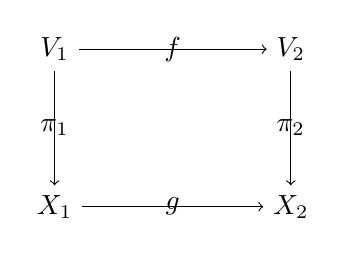
\begin{tikzpicture}
		\node (lt) {$V_1$};
		\node (rt) at (3,0) {$V_2$};
		\node (lb) at (0,-2) {$X_1$};
		\node (rb) at (3,-2) {$X_2$};
		\draw[->] (lt) to node {$f$} (rt);
		\draw[->] (lb) to node {$g$} (rb);
		\draw[->] (lt) to node [swap] {$\pi_1$} (lb);
		\draw[->] (rt) to node {$\pi_2$} (rb);
		\end{tikzpicture}
	\end{center}
	commutes and $f$ is fiberwise linear. That is, for every $x\in X_1$ the restriction of $f$ onto $\pi_1^{-1}(x)$ is a linear map between the vector spaces $\pi_1^{-1}(x)$ and $\pi_2^{-1}(g(x))$.
	
	Note that $g$ is uniquely determined by $f$.
\end{defi}

\begin{defi}[$G$\=/linearisation of a line bundle, \phantom{}{\cite[chapter 1.3]{git}}]
	Let $G$ be an affine algebraic group acting on an affine variety $X$. Let $\pi\colon L \rightarrow X$ be a line bundle over $X$. A \emph{$G$\=/linearisation of $L$} is a morphism $(f,h)$ from the line bundle $G\times L$ to $L$ such that
	$$f\colon G\times L \longrightarrow L$$
	is an algebraic group action and
	\begin{center}
		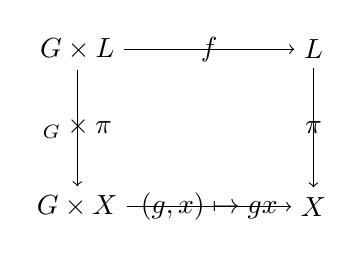
\begin{tikzpicture}
		\node (lt) {$G\times L$};
		\node (rt) at (3,0) {$L$};
		\node (lb) at (0,-2) {$G\times X$};
		\node (rb) at (3,-2) {$X$};
		\draw[->] (lt) to node {$f$} (rt);
		\draw[->] (lb) to node {$(g,x)\mapsto gx$} (rb);
		\draw[->] (lt) to node [swap] {$\id_G\times \pi$} (lb);
		\draw[->] (rt) to node {$\pi$} (rb);
		\end{tikzpicture}
	\end{center}
	commutes. A \emph{$G$\=/linearised line bundle} is a line bundle $L$ together with a  $G$\=/linearisation of $L$.
\end{defi}

\begin{remark}
	\label{remark:linearised_line_bundle_tensor}
	The tensor product $L_1 \tensor L_2$ of $G$\=/linearised line bundles $L_1$ and $L_2$ over $X$ with $G$\=/linearisations $f_1$, $f_2$ is the $G$\=/linearised line bundle that is obtained by taking the tensor product on the fibers. Its group action is given by tensoring the actions $f_1$ and $f_2$ restricted to the fibers. Note that $L_1^{\tensor n}$ is isomorphic to the line bundle $L_1$ with the $G$\=/linearisation
	$$G\times L_1 \longrightarrow L_1,\quad (g, \ell) \mapsto f_1(g^n, \ell)$$
\end{remark}

\begin{remark}[Group action on sections, \phantom{}{\cite[Remark 1.7]{git_equivalence}}]
	Let $L$ be a $G$\=/linearised line bundle over $X$. For each $G$\=/invariant open subset $U\subseteq X$ we obtain a group action of $G$ on the space $\Gamma(U,L)$ of sections of over $U$ by setting
	$$(g\cdot s)(x) \defeq g\cdot s(g^{-1}x).$$
	The identity and compatibility axioms are verified easily. We check that $g\cdot s$ again is a section in $\Gamma(U,L)$. It is well defined on $U$ since we have $g^{-1}x\in U$ for all $g\in G$, $x\in U$. Clearly, $g\cdot s$ is the composition of morphisms and thus a morphism itself.
	
	The subspace of $G$\=/invariant sections of $L$ over $U$ is denoted by $\Gamma(U,L)^G$.
	\index{GammaULG@$\Gamma(U,L)^G$}%
\end{remark}

Now we are ready to describe the construction of semistable and stable points in accordance with \cite[Definition 1.7 \& 1.8]{git}. Note that for us, stable points mean properly stable points in the sense of Mumford.

\begin{defi}
	Let $L$ be a $G$\=/linearised, ample line bundle over $X$. A point $x\in X$ is called
	\begin{enumerate}[label={\upshape(\roman*)}]
		\item \emph{semistable} if there exists a $G$\=/invariant global section $s\in\Gamma(X,L^{\tensor n})^G$ for some $n\in\natural$ such that $s(x)\neq 0$, where $0$ is the origin in the fiber $\pi^{-1}(x)$.
		\item \emph{stable} if its stabiliser $G_x$ is finite and it is semistable via a global section $s$ such that all $G$\=/orbits in 
		$$X_s = X\setminus V(s) = \{p\in X\mid s(p) \neq 0 \}$$
		are closed.
	\end{enumerate}
	The sets of semistable points and stable points are denoted by $X^{ss}(L)$ and $X^{s}(L)$ respectively.
	\index{XssL@$X^{ss}(L)$}%
	\index{XsL@$X^{s}(L)$}%
\end{defi}

\begin{remark}
	\label{remark:semistable_points_yield_git_quotient}
	By Mumford, the $G$\=/invariant set $X^{ss}(L)$ permits a good quotient $X^{ss}(L)\sslash G$, called \emph{GIT quotient}. It is the projective variety of the graded ring
	$$\bigoplus_{n\geq 0} \Gamma(X,L^{\tensor n})^G.$$
	If  $X^{s}(L)$ is non\=/empty, $X^{ss}(L)\sslash G$ is an almost geometric quotient with the restriction to $X^{s}(L)$ being a geometric quotient.
\end{remark}

\section{The GIT fan}

The set of semistable points $X^{ss}(L)$ and the corresponding GIT quotient depend on the choice of a $G$\=/linearised line bundle. As we will see in this section, we are able to parametrise all nonempty sets of semistable points arising from linearisations of the trivial line bundle by a special quasifan, called GIT fan, whose cones are in inclusion\=/reversing one\=/to\=/one correspondence. We assume that the group $G$ is an algebraic torus acting on an affine variety $X$. Note that the general case of arbitrary connected reductive groups $G$ may be reduced to the torus case, see \cite[Lemma 3.3]{git_via_cox_rings}. The concepts presented here originate from \cite[chapter 2]{git_equivalence}.

For the remainder of this section assume that $X$ is an affine variety with a $\integer^k$\=/grading on its ring $\O(X)$ of regular functions encoding an action of a $k$\=/dimensal torus $T$ by Construction~\ref{construction:algebraic_torus}.

\begin{lemma}[\phantom{}{\cite[Lemma 2.6]{git_equivalence}}]
	The $T$\=/linearisations of the trivial line bundle 
	$$\pi\colon X \times \field \rightarrow X$$
	correspond one\=/to\=/one to vectors in $\integer^k$, where $w\in\integer^k$ defines the $G$\=/linearisation
	\begin{equation}
		\label{equa:torus_linearisation}
		t\cdot(x,z) \defeq (t\cdot x, t^w z).
	\end{equation}
\end{lemma}
\begin{proof}
	One easily computes that (\ref{equa:torus_linearisation}) defines a $T$\=/linearisation for all $w\in\integer^k$. Now let $f:T\times X\times\field \rightarrow X\times\field$ be an arbitrary $T$\=/linearisation. Let $p_X$ and $p_\field$ be the projections of $X\times\field$ to $X$ and $\field$ respectively. Since $f$ is defined such that $\pi$ is equivariant, it follows that $p_X \circ f (t, x, z) = tx$. Furthermore, $p_\field \circ f(t,x,z)$ is linear w.r.t. $z$. For this reason there exists a morphism $c\colon T \times X \rightarrow \field$ such that
	$$p_\field \circ f(t,x,z)=c(t,x)z.$$
	Let $x\in X$. The compatibility axiom yields
	\begin{equation}
		\begin{aligned}
			c(t_1t_2, x) & = p_\field\circ f(t_1t_2, x, 1) \\
			& = p_\field(f(t_1, f(t_2, x, 1))) \\
			&= p_\field(f(t_1, t_2x, c(t_2,x))) \\
			&= c(t_1, t_2x)\cdot c(t_2, x).
		\end{aligned}
		\label{equa:torus_linearisation_compatibility}
	\end{equation}
	Due to the identity axiom and (\ref{equa:torus_linearisation_compatibility})
	$$1_\field = c(1_T, x) = c(t^{-1}, tx)\cdot c(t, x) \quad \forall (t,x)\in T\times X$$
	holds. In particular, $c$ does not vanish somewhere on $T\times X$, so that $c(\wildcard,x)$ becomes an invertible, rational function for every $x\in X$. By \cite[Proposition 3]{rationality_questiongs_algebraic_groups}, $c(\wildcard,x)$ is a character of $T$. As every character of $T$ is given by $t\mapsto t^\alpha$ for a suitable $\alpha\in\integer^d$ (see \cite[§16]{linear_algebraic_groups}), we conclude that 
	$$c = \sum_{\alpha\in I} t^\alpha \tensor f_\alpha \quad\text{with suitable}\ f_\alpha\in \O(X)\setminus\{0\}$$
	where for every $x\in X$ there exists exactly one $\alpha\in I$ such that $f_\alpha(x) = 1$ and $f_\beta(x) = 0$ for all $x\in I\setminus\{\alpha\}$.
	
	If $|I|>1$, we would obtain
	$$\bigcup_{\alpha\in I} V(f_\alpha) = X,$$
	contradicting the irreducibility of $X$. Thus, $I$ has to contain a single element which we denote by $w$. It follows that $c = t^w \tensor 1$.	
\end{proof}

\begin{notation}
	Let $w\in\integer^k$. We denote the $G$\=/linearised trivial line bundle corresponding to $w$ by $L_w$ and write $X(w)$ for the set of semistable points $X^{ss}(L_w)$.
	\index{Lomega@$L_w$}%
	\index{Xomega@$X(w)$}%
\end{notation}

Now that we have identified all GIT quotients arising from $T$\=/linearisations, we are going to complement them by a combinatorical description in terms of cones. A key role is assigned to orbit cones, from which finitely many exist. These contain all characters $w\in\integer^k$ of $T$ that permit a global section invariant w.r.t. to $L_w$ not vanishing on a fixed point $x\in X$. Non\=/empty intersections of orbit cones, called GIT cones, represent all non\=/empty sets of semistable points. Most interestingly, the collection of GIT cones form a quasifan with convex support. We exploit this fact later when giving an algorithmic solution for determining all GIT cones.

\begin{defi}[Orbit cone, \phantom{}{\cite[Definition 2.1]{git_equivalence}}]
	\label{defi:orbit_cone}
	Let $x\in X$. The \emph{orbit monoid} of $x$ is given by
	$$S_T(x) = \{w\in\integer^k\mid \exists f\in\O(X)_w\colon f(x) \neq 0\}.$$
	The convex, polyhedral cone $\omega_T(x)$ generated by $S_T(x)$ is called \emph{orbit cone} of $x$.
	\index{STx@$S_T(x)$}%
	\index{omegaTx@$\omega_T(x)$}%
	
	The \emph{weight cone} of $X$ is defined by
	$$\Omega_T(X) = \langle w\in\integer^k\mid \O(X)_w \neq 0 \rangle_{\real_{\geq 0}}.$$
	Clearly, the union over all orbit cones is $\Omega_T(X)$.
	\index{OmegaTX@$\Omega_T(X)$}%
\end{defi}

\begin{lemma}
	Let $x\in X$. Then $S_T(x)$ indeed is a submonoid of $\integer^k$.
\end{lemma}
\begin{proof}
	Obviously, $0\in S_T(x)$ by considering $1$ in $\O(X)$. It remains to check that $S_T(x)$ is closed. Let $w_1, w_2\in S_T(x)$. Hence, there exist $f_1\in\O(X)_{w_1}$ and $f_2\in\O(X)_{w_2}$ with $f_1(x) \neq 0 \neq f_2(x)$.
	The product $f_1f_2$ is homogeneous of degree $w_1+w_2$ with $(f_1f_2)(x) \neq 0$. We conclude that $w_1+w_2\in S_T(x)$.
\end{proof}

\begin{prop}[\phantom{}{\cite[Proposition 2.5]{git_equivalence}}]
	\label{prop:finite_orbit_cones}
	The collection of orbit cones $\{\omega_T(x)\mid x\in X\}$ is finite.
\end{prop}
\begin{proof}
	By Construction~\ref{construction:algebraic_torus}, we can embed $X$ into a suitable affine space $\field^m$ such that $\O(X)$ becomes the ring $\field[\mathbf{x}]/I(X)$ with grading
	$$\deg(x_i) = q_i\in\integer^k\quad\forall 1\leq i \leq m.$$
	Let $x\in X$ and $w\in\integer^k$ such that $w\in S_T(x)$. Then there exists a polynomial $f\in\field[\mathbf{x}]$ of degree $w$ with $f(x)\neq 0$. It follows that $f$ contains at least one monomial $\mathbf{x}^\alpha$ of degree $w$ that does not vanish when substituting $x$. In particular
	$$(t *_{(\field^*)^m} x)^\alpha = t^\alpha \cdot x^\alpha \neq 0$$
	for $t\in(\field^*)^m$, where $*_{(\field^*)^m}$ denotes the standard action of $(\field^*)^m$ on $\field^m$. We conclude that $S_T(x)$ is constant on $(\field^*)^m$\=/orbits over $\field^m$. Since there exist only a finite number of such orbits, the claim follows.
\end{proof}

\begin{lemma} Let $w\in\integer^k$. Then it holds that
	\label{lemma:semistable_points_determined_by_orbit_cones}
	\begin{align*}
	X(w) 
	&= \bigcup_{f\in\O(X)_{nw},\ n\in\natural} X_f\\
	&= \{x\in X\mid w\in\omega_T(x)\}.
	\end{align*}
\end{lemma}
\begin{proof}
	By Remark~\ref{remark:linearised_line_bundle_tensor}, we have $L_w^{\tensor n} = L_{nw}$ for all $n\in\natural$. Now fix $n\in\natural$ and let $s\in\Gamma(X,L_{nw})$ be a global section. Since we consider the (ample) trivial line bundle, $s$ corresponds to a morphism $f\in\O(X)$ such that
	$$s(x) = (x, f(x))\quad \forall x\in X.$$
	and $X_f$ contains all points with $s(x) \neq 0$. The section is $G$\=/invariant iff
	$$(tx, (t^{-1}f)(x)) = (tx, f(tx)) = s(tx) = (t\cdot s)(tx) = t\cdot s(x) = (tx, t^{nw} f(x))$$
	for all $t\in T$, $x\in X$. Taking Example~\ref{example:regular_functions_torus_group_action} into account, we obtain
	$$s\in\Gamma(X,L_{nw})^G \ \Longleftrightarrow\ f\in\O(X)_{nw}$$
	and the first equation follows. The inclusion $\subseteq$ of the second equation is obvious. For the other direction, let $x\in X$ such that $w\in\omega_T(x)$. After eliminating denominators in a $\rational$\=/linear combination of $w$ over $S_T(x)$, one obtains $n\in\natural$ such that $nw \in S_T(x)$. The inclusion $\supseteq$ follows.
\end{proof}

\begin{coro} Let $w\in\integer^k$. The following conditions are equivalent:
	\begin{enumerate}[label={\upshape(\roman*)}]
	\item $X(w) \neq \emptyset$,
	\item $w\in\Omega_T(X)$.
	\end{enumerate}
\end{coro}
\begin{proof}
	Immediate consequence of Lemma~\ref{lemma:semistable_points_determined_by_orbit_cones} and the definition of the weight cone $\Omega_T(X)$.
\end{proof}

\begin{defi}[GIT cone, \phantom{}{\cite[Definition 2.8]{git_equivalence}}]
Let $w\in\Omega_T(X)$. The \emph{GIT cone} associated to $w$ is defined by
$$\sigma_T(w) = \bigcap_{w\in\omega_T(x)} \omega_T(x).$$
\index{sigmaTw@$\sigma_T(w)$}%

The collection of all GIT cones
$$\Sigma_T(X) \defeq \{\sigma_T(w)\mid w\in\Omega_T(X)\}$$
is called \emph{GIT fan}.
\index{SigmaTX@$\Sigma_T(X)$}%
\end{defi}

\begin{prop}[\phantom{}{\cite[Proposition 2.9]{git_equivalence}}]
	\label{prop:equivalence_git_cones_semistable_points}
	Let $w_1, w_2\in \Omega_T(x)$. Then
	$$X(w_1)\subseteq X(w_2) \ \Longleftrightarrow\ \sigma_T(w_1) \supseteq \sigma_T(w_2).$$
	In particular, $X(w_1) = X(w_2)$ if and only if $\sigma_T(w_1) = \sigma_T(w_2)$.
\end{prop}
\begin{proof}
	By Lemma~\ref{lemma:semistable_points_determined_by_orbit_cones} and the definition of GIT cones, for any $v,w\in\integer^k$ we have
	\begin{align*}
		v\in\sigma_T(w) &\ \Leftrightarrow\ v\in \omega_T(x)\quad \forall x\in X\ \mathrm{with}\ w\in\omega_T(x) \\
		&\ \Leftrightarrow\ v\in \omega_T(x)\quad \forall x\in X(w).
	\end{align*}
	The direction $\Rightarrow$ follows. For the converse, consider $X(w_1) \nsubseteq X(w_2)$ so that there exists $x\in X$ with $w_1\in \omega_T(x)$ and $w_2\notin \omega_T(x)$ by Lemma~\ref{lemma:semistable_points_determined_by_orbit_cones}. Since $\sigma_T(w_1)$ is a subset of $\omega_T(x)$, we conclude that $w_2\notin\sigma_T(w_1)$ and therefore $\sigma_T(w_2)\nsubseteq\sigma_T(w_1)$.
	
	The postscript immediately follows from the first claim.
\end{proof}

\begin{theorem}[\phantom{}{\cite[Theorem 2.11]{git_equivalence}}]
	\label{theorem:git_fan}
	The GIT fan $\Sigma_T(X)$ is a quasifan, that is a finite collection of convex polyhedral cones located in the same ambient space such that for $\sigma, \sigma'\in \Sigma_T(X)$
	\begin{enumerate}[label={\upshape(\roman*)}]
		\item all faces of $\sigma$ belong to $\Sigma_T(X)$,
		\item $\sigma \cap \sigma'$ is a face of both $\sigma$ and $\sigma'$.
	\end{enumerate}
	Its support $\cup_{\sigma\in\Sigma_T(X)}\sigma$ is given by the (convex) weight cone $\Omega_T(X)$.
\end{theorem}

We postpone the proof and begin with some lemmas. Since the closure of a $T$\=/orbit in $X$ is $T$\=/invariant, it decomposes into a set of (possibly non\=/closed) $T$\=/orbits. The following lemma translates this setup into the world of orbit cones. We omit the proof and refer to \cite{git_equivalence}.

\begin{lemma}[\phantom{}{\cite[Corollary 2.4]{git_equivalence}}]
	\label{lemma:orbits_correspond_to_orbit_cones}
	The $T$\=/orbits in $X$ are in one\=/to\=/one correspondence with orbit cones via
	$$Ty \mapsto \omega_T(y).$$
	
	Let $x\in X$. Then all faces of $\omega_T(x)$ are orbit cones such that $\omega_T(y)$ is a face if and only if the corresponding $T$\=/orbit $Ty$ is located in $\overline{Tx}$.
\end{lemma}

\begin{notation}
	Let $\sigma\subseteq \real^k$ be a cone. We write $\sigma^\circ$ for the relative interior of $\sigma$. Note that if $\sigma$ is of full dimension $k$, then the interior of $c$ w.r.t. the euclidean topology coincides with the relative interior $\sigma^\circ$.
	\index{sigma°@$\sigma^\circ$}%
\end{notation}

\begin{lemma}[\phantom{}{\cite[Lemma 2.12]{git_equivalence}}]
	\label{lemma:git_cones_alternative_descriptions}
	Let $w\in\Omega	_T(X)$. Then it holds that
	\begin{enumerate}[label={\upshape(\roman*)}]
		\item $w\in \omega_T(x) \ \Leftrightarrow\ \sigma_T(w) \subseteq \omega_T(x)\quad \forall x\in X,$
		\label{enum_item:git_cone_in_all_orbit_cones}
		\item $w\in \omega_T(x)^\circ \ \Leftrightarrow\ \sigma_T(w)^\circ \subseteq \omega_T(x)^\circ\quad \forall x\in X,$
		\label{enum_item:git_cone_interior_in_all_orbit_cone_interiors}
		\item $\sigma_T(w) = \bigcap\limits_{w\in \omega_T(x)^\circ} \omega_T(x),$
		\label{enum_item:git_cone_intersection_wrt_interiors}
		\item $\sigma_T(w)^\circ = \bigcap\limits_{w\in \omega_T(x)^\circ} \omega_T(x)^\circ,$
		\label{enum_item:git_cone_interior}
		\item $w\in\sigma_T(w)^\circ.$
		\label{enum_item:git_cone_generator_in_interior}
	\end{enumerate}
\end{lemma}
\begin{proof}
	\ref{enum_item:git_cone_in_all_orbit_cones} immediately follows from the definition of GIT cones.
	
	For any orbit cone $\omega_T(x)$ with $w\in\omega_T(x)$ there exists a minimal face $\omega\preceq \omega_T(x)$ containing $w$ in its relative interior. Since $\omega$ is an orbit cone by Lemma~\ref{lemma:orbits_correspond_to_orbit_cones}, it suffices to intersect with orbit cones containing $w$ in its interior, showing \ref{enum_item:git_cone_intersection_wrt_interiors}.
	
	\ref{enum_item:git_cone_interior} and \ref{enum_item:git_cone_generator_in_interior} are a consequence of the following fact: If the intersection of the relative interiors of a finite number of convex polyhedral cones is non\=/empty, then it equals the relative interior of the intersection of the cones. \ref{enum_item:git_cone_interior_in_all_orbit_cone_interiors} follows from \ref{enum_item:git_cone_interior} and \ref{enum_item:git_cone_generator_in_interior}.
\end{proof}

\begin{lemma}[\phantom{}{\cite[Proof of Theorem 2.11]{git_equivalence}}]
	\label{lemma:git_cone_subsets_of_git_cones_are_faces}
	Let $w_1,w_2\in\Omega_T(X)$. Then the inclusion $\sigma_T(w_1) \subseteq \sigma_T(w_2)$ implies $\sigma_T(w_1) \preceq \sigma_T(w_2)$.
\end{lemma}
\begin{proof}
	 Let $\omega_T(x_1),\dots,\omega_T(x_r)$ be the orbit cones with $\sigma_T(w_1)^\circ \subseteq \omega_T(x_i)^\circ$ for $1\leq i \leq r$. By Lemma~\ref{lemma:git_cones_alternative_descriptions}, we have $\sigma_T(w_1) = \omega_T(x_1) \cap \cdots \cap \omega_T(x_r)$.
	 
	 Choose representatives $x_1,y_1,\dots,y_\ell$ of the $T$\=/orbit decomposition of $\overline{Tx_1}$.
	 Then Lemma~\ref{lemma:orbits_correspond_to_orbit_cones} states that $\omega_T(y_i) \preceq \omega_T(x_1)$ is a proper face for all $1\leq i \leq \ell$. Because of $\sigma_T(w_1)^\circ \subseteq \omega_T(x_1)^\circ$, it follows that $\omega_T(y_i) \cap \sigma_T(w_1)^\circ = \emptyset$. By Lemma~\ref{lemma:git_cones_alternative_descriptions}, $w_1$ is contained in $\sigma_T(w_1)^\circ$ but not in $\omega_T(y_i)$. For this reason $y_i\notin X(w_1)$ holds. Together with $x_1\in X(w_1)$ due to $w_1\in \sigma_T(w_1)^\circ \subseteq \omega_T(x_1)^\circ$, we conclude that
	 \begin{equation}
		 \label{equa:orbit_closed_in_Xw1}
		 \overline{Tx_1} \cap X(w_1) = Tx_1,
	 \end{equation}
	 i.e. $Tx_1$ is closed in $X(w_1)$.
	 
	 By Proposition~\ref{prop:equivalence_git_cones_semistable_points}, we have $X(w_2)\subseteq X(w_1)$. We denote the good quotient maps of $X(w_1)$ and $X(w_2)$ by $p_1$ and $p_2$ respectively. The morphism
	 $$\varphi: X(w_2) \hookrightarrow X(w_1) \rightarrow X(w_1) \sslash T$$
	 is $G$\=/invariant. Hence, the universal property of categorical quotients yields a unique morphism $\psi: X(w_2)\sslash T \rightarrow X(w_1)\sslash T$ such that the diagram
	 \begin{center}
	 	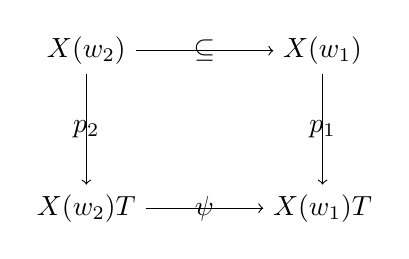
\begin{tikzpicture}
	 	\node (lt) {$X(w_2)$};
	 	\node (rt) at (3,0) {$X(w_1)$};
	 	\node (lb) at (0,-2) {$X(w_2) \sslash T$};
	 	\node (rb) at (3,-2) {$X(w_1) \sslash T$};
	 	\draw[->] (lt) to node {$\subseteq$} (rt);
	 	\draw[->] (lb) to node {$\psi$} (rb);
	 	\draw[->] (lt) to node [swap] {$p_2$} (lb);
	 	\draw[->] (rt) to node {$p_1$} (rb);
	 	\end{tikzpicture}
	 \end{center}
	 commutes. Since both $X(w_1) \sslash T$ and $X(w_2) \sslash T$ are projective over $\O(X)_0$ due to Remark~\ref{remark:semistable_points_yield_git_quotient}, $\psi$ is projective with closed image in $X(w_1) \sslash T$. Furthermore, $X(w_2)$ is a $G$\=/invariant, dense open subset of $X(w_1)$. By the definition of good quotients, the image of the closed complement $X(w_1)\setminus X(w_2)$ under $p_1$ is closed. Proposition~\ref{prop:good_quotient_properties} shows that $p_1$ is surjective, so that the image of $X(w_2)$ under $p_1$, which is the image of $\psi$, contains a non\=/empty open subset and thus is dense. Overall it follows that $\psi$ is surjective. 
	 
	 Now, there exists a point $z_1\in X(w_2) \cap p_1^{-1}(p_1(x_1))$. By Proposition~\ref{prop:good_quotient_properties}, it follows that 
	 $$\overline{Tx_1} \cap \overline{Tz_1} \cap X(w_1) \neq \emptyset.$$
	 Applying (\ref{equa:orbit_closed_in_Xw1}) yields
	 $$Tx_1 \cap \overline{Tz_1} \neq \emptyset$$
	 which results in
	 $$Tx_1 \subseteq \overline{Tz_1}.$$
	 By Lemma~\ref{lemma:orbits_correspond_to_orbit_cones}, $\omega_T(x_1)$ is a face of $\omega_T(z_1)$. Because of $z_1\in X(w_2)$, it holds that $w_2\in \omega_T(z_1)$, that is $\sigma_T(w_2) \subseteq \omega_T(z_1)$ by Lemma~\ref{lemma:git_cones_alternative_descriptions}. Repeating the process for $x_2,\dots,x_r$ yields orbit cones $\omega_T(z_i)$ such that $\omega_T(x_i)\preceq \omega_T(z_i)$ and $\sigma_T(w_2) \subseteq \omega_T(z_i)$ for all $1\leq i\leq r$.
	 
	 Now let $\tau\preceq \sigma_T(w_2)$ be the unique face with $\sigma_T(w_1)^\circ \subseteq \tau^\circ$ by Lemma~\ref{lemma:cones_in_cones}. In particular,
	 $$\tau\subseteq\omega_T(z_i)\quad\mathrm{and}\quad\emptyset \neq \sigma_T(w_1)^\circ \subseteq \tau^\circ \cap \omega_T(x_i)^\circ$$
	 hold for all $1\leq i\leq r$. Again by Lemma~\ref{lemma:cones_in_cones}, we conclude that $\tau\subseteq \omega_T(x_i)$. It follows that $\tau \subseteq \sigma_T(w_1)$. The equality is obtained by taking closures in $\sigma_T(w_1)^\circ \subseteq \tau^\circ$. Hence, $\sigma_T(w_1) = \tau$ is a face of $\sigma_T(w_2)$.
\end{proof}

Now we are ready to proof Theorem~\ref{theorem:git_fan}.
\begin{proof}
	The finiteness of $\Sigma_T(X)$ is an immediate consequence of Proposition~\ref{prop:finite_orbit_cones}. 
	
	Let $\sigma\in\Sigma_T(X)$ be a GIT cone and $\sigma_0\preceq\sigma_T(w)$ be a face. Choose $w\in\sigma_0^\circ$. By Lemma~\ref{lemma:git_cones_alternative_descriptions}, $\sigma$ is the intersection of all orbit cones containing $\sigma$. These also contain $w$, hence $\sigma_T(w)\subseteq \sigma$ by the definition of GIT cones. The prerequisite of Lemma~\ref{lemma:git_cone_subsets_of_git_cones_are_faces} is satisfied so that $\sigma_T(w)\preceq \sigma$. Now, $\sigma_T(w)$ and $\sigma_0$ are both faces of $\sigma$ containing $w$ in their relative interior by Lemma~\ref{lemma:git_cones_alternative_descriptions}. This may only be the case when $\sigma_0 = \sigma(w)$, proving that $\sigma_0\in\Sigma_T(X)$.
	
	Next, let $\sigma_1,\sigma_2\in\Sigma_T(X)$. Let $\tau_i\preceq\sigma_i$ be the unique face such that $(\sigma_1\cap\sigma_2)^\circ \subseteq \tau_i^\circ$ by Lemma~\ref{lemma:cones_in_cones} ($i=1,2$). Let $w\in(\sigma_1\cap\sigma_2)^\circ$. In particular, it holds that $w\in\tau_i^\circ$, so that we obtain $\sigma(w) = \tau_i$ and $\sigma(w)\subseteq \sigma_i$ as before. Due to $\sigma_1 \cap \sigma_2 \subseteq \tau_i$, it follows that 
	$$\sigma_1 \cap \sigma_2 = \tau_1 = \tau_2 = \sigma(w).$$
	For this reason, $\sigma_1 \cap \sigma_2$ is a face of both $\sigma_1$ and $\sigma_2$.
\end{proof}

\section{Mori dream spaces, movable divisor classes?}